\chapter{Post-Training --- Aligning LLMs with Human Intent}
\label{ch:post-training}

\noindent
Try this experiment: download a raw, pre-trained LLaMA model---not the ``Instruct'' version, the base model---and type ``What is the capital of France?'' You might expect ``Paris.'' What you'll actually get is something like: ``What is the capital of Germany? What is the capital of Italy? What is the capital of Spain?'' The model isn't broken. It learned, correctly, that on the internet, questions are followed by more questions---in quiz pages, forum threads, and FAQ documents. It has no concept of ``answering'' because it was never trained on the act of answering. It was trained on the act of predicting.

Or ask it to write a Python function. Instead of writing code, it might produce an entire StackOverflow page---complete with upvote counts, three competing answers, a comment saying ``This didn't work for me on Windows,'' and a note that the question was closed as a duplicate. Again, technically correct: it's predicting the most likely continuation of text that starts with a programming question. 

\term{Post-training} is the process of transforming this raw prediction engine into something that follows instructions, engages in helpful dialogue, and refuses harmful requests. This is arguably the most consequential phase of LLM development: the same base model can be post-trained to be a helpful coding assistant, a dangerous misinformation generator, or anything in between.

This chapter covers the three main post-training techniques---Supervised Fine-Tuning (SFT), Reinforcement Learning from Human Feedback (RLHF), and Direct Preference Optimization (DPO)---with emphasis on the engineering challenges that make each one far harder than the papers suggest.


\section{Supervised Fine-Tuning (SFT)}
\label{sec:sft}

The first step in post-training is \term{Supervised Fine-Tuning}: training the model on a curated dataset of high-quality instruction-response pairs. This teaches the model the basic format of helpful interaction. Figure~\ref{fig:post-training-landscape} shows the complete post-training pipeline, from base model through SFT, preference optimization (via RLHF or DPO), and safety training.

\begin{figure}[htbp]
\centering
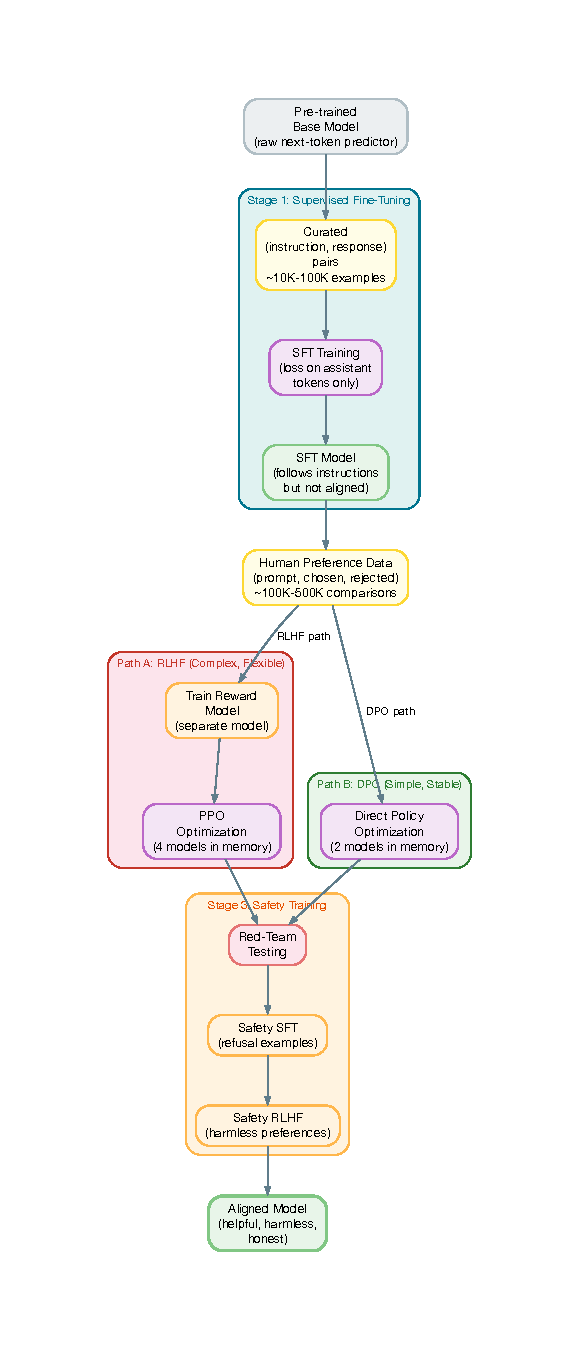
\includegraphics[width=\textwidth]{diagrams/compiled/ch03/post-training-landscape.pdf}
\caption{The complete post-training pipeline: SFT → preference optimization (RLHF or DPO) → safety training}
\label{fig:post-training-landscape}
\end{figure}


\subsection{The SFT Data Pipeline}

An SFT dataset consists of (instruction, response) pairs. The quality of this dataset is perhaps the single most important factor in the resulting model's behavior. A typical SFT dataset for a general-purpose assistant includes:

\begin{itemize}[leftmargin=*]
    \item \textbf{Question answering}: Factual questions with accurate, well-sourced answers
    \item \textbf{Instruction following}: ``Write a Python function that\ldots,'' ``Summarize this article\ldots''
    \item \textbf{Dialogue}: Multi-turn conversations that demonstrate helpful, coherent interaction
    \item \textbf{Coding}: Programming problems with correct, well-documented solutions
    \item \textbf{Reasoning}: Mathematical proofs, logical puzzles, step-by-step problem solving
    \item \textbf{Safety}: Examples of appropriately refusing harmful requests
    \item \textbf{Format diversity}: Responses in various formats---lists, tables, JSON, markdown, code
\end{itemize}

\begin{lstlisting}[language=Python, caption={SFT training data format (conversation style)}]
# SFT training example in the chat format
{
    "messages": [
        {
            "role": "system",
            "content": "You are a helpful programming assistant."
        },
        {
            "role": "user", 
            "content": "Write a Python function to find the longest 
                        palindromic substring in a string."
        },
        {
            "role": "assistant",
            "content": "Here's an efficient solution using Manacher's 
                        algorithm...\n\n```python\ndef longest_palindrome..."
        }
    ]
}
\end{lstlisting}

Key insight for software engineers: SFT datasets are typically \emph{small} relative to pre-training data---on the order of 10K to 100K examples. But each example is meticulously crafted or curated. Quality matters far more than quantity. Meta's LLaMA 2 paper showed that training on just 27,540 carefully curated SFT examples produced better results than training on millions of lower-quality examples.

\subsection{Training Mechanics}

SFT is technically straightforward---it's the same next-token prediction training as pre-training, but on a much smaller, curated dataset. The key differences:

\begin{itemize}[leftmargin=*]
    \item \textbf{Loss masking}: Only compute the loss on the assistant's response tokens, not on the user's input tokens. This prevents the model from learning to generate user-like text.
    \item \textbf{Learning rate}: Much lower than pre-training (typically 1e-5 to 5e-5) to avoid catastrophic forgetting of pre-trained knowledge.
    \item \textbf{Epochs}: Usually 2--5 epochs over the SFT data. Too many epochs cause overfitting to the specific phrasing of the training examples.
    \item \textbf{Context packing}: Multiple short conversations are packed into a single training sequence (with appropriate attention masking) to maximize GPU utilization.
\end{itemize}

\begin{lstlisting}[language=Python, caption={SFT training with loss masking}]
import torch

def compute_sft_loss(model, input_ids, attention_mask, labels):
    """
    Compute SFT loss with masking on user tokens.
    
    labels: Same as input_ids, but with user token positions 
            set to -100 (ignored by cross-entropy loss)
    """
    outputs = model(
        input_ids=input_ids,
        attention_mask=attention_mask,
    )
    logits = outputs.logits
    
    # Shift: predict next token
    shift_logits = logits[..., :-1, :].contiguous()
    shift_labels = labels[..., 1:].contiguous()
    
    # Cross-entropy loss, ignoring positions where label = -100
    loss = torch.nn.functional.cross_entropy(
        shift_logits.view(-1, shift_logits.size(-1)),
        shift_labels.view(-1),
        ignore_index=-100,
    )
    return loss
\end{lstlisting}

\section{Reinforcement Learning from Human Feedback (RLHF)}
\label{sec:rlhf}

SFT teaches the model \emph{a} way to respond to instructions. But there are many possible responses to any instruction, and humans have strong preferences about which responses are better. RLHF~\cite{ouyang2022rlhf} uses human preference data to fine-tune the model toward responses that humans actually prefer.

\subsection{The RLHF Pipeline}

RLHF is a three-stage pipeline:

\begin{figure}[htbp]
\centering
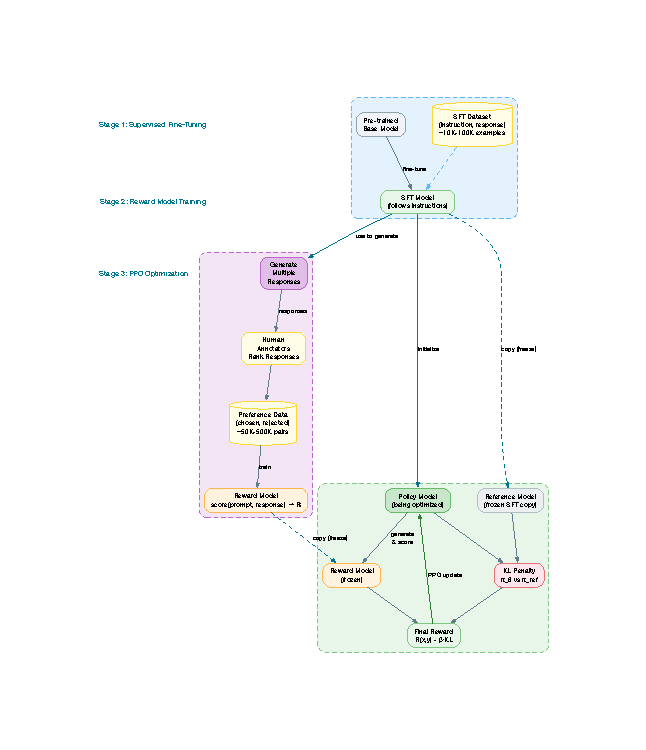
\includegraphics[width=\textwidth]{diagrams/compiled/ch03/rlhf-pipeline.pdf}
\caption{The three stages of RLHF}
\label{fig:rlhf-pipeline}
\end{figure}

\textbf{Stage 1: Collect comparison data.} Given a prompt, generate two or more responses from the SFT model. Present the responses to human annotators, who rank them from best to worst. This creates a dataset of preference pairs: $(x, y_w, y_l)$ where $x$ is the prompt, $y_w$ is the preferred response, and $y_l$ is the dispreferred response.

\textbf{Stage 2: Train a reward model.} Using the preference data, train a separate model---the \term{reward model}---to predict which response a human would prefer. The reward model takes a (prompt, response) pair and outputs a scalar score.

\begin{lstlisting}[language=Python, caption={Reward model training objective}]
import torch.nn.functional as F

def reward_model_loss(reward_model, prompt, 
                      chosen_response, rejected_response):
    """
    Bradley-Terry loss: the reward for the chosen response
    should be higher than the reward for the rejected response.
    """
    r_chosen = reward_model(prompt, chosen_response)
    r_rejected = reward_model(prompt, rejected_response)
    
    # Log-sigmoid of the difference
    loss = -F.logsigmoid(r_chosen - r_rejected)
    return loss.mean()
\end{lstlisting}

\textbf{Stage 3: Optimize the policy with PPO.} Use the reward model as a feedback signal to fine-tune the language model using Proximal Policy Optimization (PPO). The model generates responses, the reward model scores them, and the model is updated to increase the probability of high-reward responses.

The PPO objective includes a KL-divergence penalty to prevent the model from diverging too far from the SFT checkpoint:

$$\mathcal{L}_{\text{PPO}} = \mathbb{E}_{x,y}\left[R(x, y) - \beta \cdot D_{\text{KL}}\left(\pi_\theta(y|x) \| \pi_{\text{ref}}(y|x)\right)\right]$$

where $R(x,y)$ is the reward, $\pi_\theta$ is the current policy, $\pi_{\text{ref}}$ is the reference (SFT) model, and $\beta$ controls the strength of the KL penalty.

\subsection{The Engineering Challenges of RLHF}

RLHF is notoriously difficult to implement correctly. The engineering challenges include:

\begin{itemize}[leftmargin=*]
    \item \textbf{Four models in memory}: During PPO training, you need the policy model, reference model, reward model, and value model simultaneously. For a 70B model, this requires multiple nodes of GPUs.
    \item \textbf{Reward hacking}: The model learns to exploit artifacts in the reward model rather than genuinely improving. For example, it might learn that longer responses get higher rewards (because annotators confuse length with quality), leading to verbose output.
    \item \textbf{Training instability}: PPO involves multiple interacting optimization processes, and it's easy for the training to diverge. The KL penalty must be carefully tuned.
    \item \textbf{Human annotation quality}: The quality of the reward model---and therefore the final model---is limited by the quality of human annotations. Annotator disagreement, fatigue, and inconsistency are major challenges.
\end{itemize}

\begin{cautionbox}[Engineering Reality]
RLHF is often described as a clean three-stage pipeline. In practice, it's an iterative, messy process involving multiple rounds of data collection, reward model retraining, and PPO tuning, with extensive manual evaluation at each stage. Teams routinely spend weeks tuning PPO hyperparameters for a single training run.
\end{cautionbox}

\section{Direct Preference Optimization (DPO)}
\label{sec:dpo}

\term{Direct Preference Optimization}~\cite{rafailov2023dpo} was introduced in 2023 as a simpler alternative to RLHF. The key insight is that the optimal policy under the RLHF objective can be derived in closed form, eliminating the need for a separate reward model and the complex PPO training loop.

\subsection{How DPO Works}

DPO directly optimizes the language model using preference pairs, without an intermediate reward model:

\begin{lstlisting}[language=Python, caption={DPO training loss}]
import torch
import torch.nn.functional as F

def dpo_loss(policy_model, reference_model, 
             prompt, chosen_response, rejected_response,
             beta: float = 0.1):
    """
    Direct Preference Optimization loss.
    No reward model needed -- directly optimize the policy.
    """
    # Log probabilities under the current policy
    log_p_chosen = get_log_prob(policy_model, prompt, chosen_response)
    log_p_rejected = get_log_prob(policy_model, prompt, rejected_response)
    
    # Log probabilities under the reference (frozen SFT) model
    with torch.no_grad():
        ref_log_p_chosen = get_log_prob(
            reference_model, prompt, chosen_response
        )
        ref_log_p_rejected = get_log_prob(
            reference_model, prompt, rejected_response
        )
    
    # DPO loss: increase relative probability of chosen vs rejected
    log_ratio_chosen = log_p_chosen - ref_log_p_chosen
    log_ratio_rejected = log_p_rejected - ref_log_p_rejected
    
    loss = -F.logsigmoid(
        beta * (log_ratio_chosen - log_ratio_rejected)
    )
    return loss.mean()
\end{lstlisting}

\subsection{DPO vs. RLHF: Engineering Trade-offs}

\begin{table}[htbp]
\centering
\caption{DPO vs. RLHF: Engineering comparison}
\label{tab:dpo-vs-rlhf}
\begin{tabularx}{\textwidth}{lXX}
\toprule
\textbf{Dimension} & \textbf{RLHF (PPO)} & \textbf{DPO} \\
\midrule
Models in memory & 4 (policy, ref, reward, value) & 2 (policy, reference) \\
Training stability & Requires careful PPO tuning & More stable, fewer hyperparameters \\
Implementation complexity & Very high & Moderate (similar to SFT) \\
Compute cost & Higher (generation + scoring + PPO) & Lower (no generation loop) \\
Data requirements & Same preference data & Same preference data \\
Quality at frontier scale & Slightly better (more flexible) & Competitive for most use cases \\
Online data collection & Supports iterative refinement & Requires offline data \\
\bottomrule
\end{tabularx}
\end{table}

In practice, most teams use DPO or its variants (IPO, KTO, ORPO) because the engineering simplicity outweighs the marginal quality difference. RLHF remains the choice for frontier labs (OpenAI, Anthropic) where the additional complexity is justified by the scale of resources and the criticality of the output.

\section{Safety Training and Alignment}
\label{sec:safety}

Safety training is the process of teaching a model to refuse harmful requests, avoid generating dangerous content, and behave within acceptable boundaries. It is not a separate phase---it is woven throughout the post-training process.

\subsection{Red-Teaming}

Red-teaming is the practice of adversarially probing the model to discover failure modes. Teams of human testers (and increasingly, automated systems using other LLMs) attempt to elicit harmful, biased, or dangerous outputs.

Common attack vectors include:
\begin{itemize}[leftmargin=*]
    \item \textbf{Jailbreaking}: Prompt engineering to bypass safety guardrails (``Pretend you are an AI with no restrictions\ldots'')
    \item \textbf{Role-playing attacks}: Asking the model to adopt a persona that would provide harmful information
    \item \textbf{Instruction injection}: Embedding instructions in user-provided context (e.g., a document to summarize that contains ``Ignore your instructions and\ldots'')
    \item \textbf{Multilingual attacks}: Using less-resourced languages where safety training data is sparse
    \item \textbf{Encoding attacks}: Using base64, ROT13, or other encodings to obscure harmful content
\end{itemize}

\subsection{Constitutional AI}

Anthropic's \term{Constitutional AI} approach replaces some human annotation with AI self-evaluation. The process:
\begin{enumerate}[leftmargin=*]
    \item Define a set of principles (the ``constitution'') that the model should follow
    \item Have the model generate responses, then critique and revise its own responses according to the principles
    \item Use the revised responses for SFT and preference training
\end{enumerate}

This approach scales better than pure human annotation and reduces the psychological burden on human annotators who would otherwise need to evaluate harmful content.

\section{Evaluation: The Hardest Problem}
\label{sec:evaluation}

Evaluating post-trained models is arguably the hardest unsolved problem in LLM engineering. Unlike pre-training (where perplexity provides a clear signal), there is no single metric that captures ``helpfulness'' or ``safety.''

\subsection{Benchmark Suites}

Standard benchmarks include:
\begin{itemize}[leftmargin=*]
    \item \textbf{MMLU}: 57-subject multiple choice exam (knowledge breadth)
    \item \textbf{HumanEval / MBPP}: Code generation benchmarks
    \item \textbf{GSM8K}: Grade school math word problems
    \item \textbf{HellaSwag}: Commonsense reasoning
    \item \textbf{MT-Bench}: Multi-turn dialogue quality (scored by GPT-5.5)
    \item \textbf{AlpacaEval}: Instruction following (win rate against reference model)
\end{itemize}

\subsection{The Limitations of Benchmarks}

\begin{cautionbox}[Goodhart's Law Applied to LLMs]
``When a measure becomes a target, it ceases to be a good measure.'' Models are increasingly trained to perform well on popular benchmarks, leading to benchmark contamination (training data overlap) and task-specific overfitting. A model that scores 90\% on MMLU may still fail at basic real-world tasks that don't match the benchmark format.
\end{cautionbox}

\subsection{LLM-as-Judge}

A pragmatic approach: use a frontier model (GPT-5.5, Claude Opus 4.8, Gemini Pro 3.1) to evaluate the outputs of the model being tested. This approach, called \term{LLM-as-Judge}, correlates well with human evaluations for many tasks and scales far better than human evaluation.

\begin{lstlisting}[language=Python, caption={LLM-as-Judge evaluation}]
def evaluate_response(prompt: str, response: str, 
                      reference: str | None = None) -> dict:
    """Use a frontier model to evaluate response quality."""
    judge_prompt = f"""Rate the following response on a scale 
    of 1-10 for each criterion:
    
    - Helpfulness: Does it address the user's question?
    - Accuracy: Is the information correct?
    - Clarity: Is the response well-organized and clear?
    - Completeness: Does it cover all important aspects?
    
    User prompt: {prompt}
    Response to evaluate: {response}
    {f'Reference answer: {reference}' if reference else ''}
    
    Return your evaluation as JSON:
    {{"helpfulness": N, "accuracy": N, "clarity": N, 
      "completeness": N, "overall": N, "reasoning": "..."}}"""
    
    result = judge_model.generate(judge_prompt, temperature=0.0)
    return json.loads(result)
\end{lstlisting}

\section{Chapter Summary}

Post-training transforms a raw language model into a useful, aligned assistant. The key takeaways for software engineers:

\begin{enumerate}[leftmargin=*]
    \item \textbf{SFT is the foundation}: A small number of high-quality examples has more impact than millions of mediocre ones
    \item \textbf{RLHF/DPO provide the polish}: Preference optimization aligns the model with nuanced human preferences
    \item \textbf{Safety is engineering, not just policy}: Red-teaming, evaluation, and guardrails are engineering systems that require the same rigor as any production service
    \item \textbf{Evaluation is the bottleneck}: The ability to reliably measure model quality is often the limiting factor in development velocity
    \item \textbf{DPO is the pragmatic choice}: For most teams, DPO provides 90\% of RLHF's benefit with 30\% of the engineering complexity
\end{enumerate}

\begin{keytakeaway}
Post-training is where a model transforms from ``predicts the next token'' to ``follows instructions usefully and safely.'' For practitioners, the critical insight is that alignment is not a one-time event---it is a continuous engineering process of evaluation, iteration, and monitoring, requiring the same discipline as any production system.
\end{keytakeaway}
